\documentclass[UTF8,fontset=fandol]{ctexart}
\usepackage[a4paper,margin=1in]{geometry}
\usepackage{amsmath}
\usepackage{amssymb}
\usepackage{amsthm}
\usepackage{bm}
\usepackage{graphicx}
\usepackage{hyperref}

\newtheorem{theorem}{定理}
\newtheorem{proposition}{命题}
\newtheorem{corollary}{推论}
\theoremstyle{remark}
\newtheorem{remark}{说明}

\title{多模型预训练特征融合的理论说明}
\author{}
\date{}

\begin{document}

\maketitle

\section{问题设定}

设预训练模型池为
\[
\mathcal M = \{m_1, \dots, m_M\}.
\]
每个模型 $m$ 对输入 $x \in \mathcal X$ 输出冻结特征
\[
f_m(x) \in \mathbb R^{d_m}.
\]
对任意子集 $S \subseteq \mathcal M$，定义拼接特征
\[
F_S(x) = \bigoplus_{m \in S} f_m(x), \qquad d_S = \sum_{m \in S} d_m.
\]

目标任务标签记为随机变量 $Y$。在目标训练集
\[
s = \{(x_i, y_i)\}_{i=1}^n \sim P^{\otimes n}
\]
上，我们只训练轻量分类头或轻量融合器，而预训练编码器保持冻结。

本文主要回答两个问题：
\begin{itemize}
    \item 为什么更多模型在总体层面不会让 Bayes 最优变差，但在有限样本下却可能使准确率先上升后下降？
    \item 为什么模型排序不能只看多样性，而必须同时考虑任务相关性与类条件修正项？
\end{itemize}

\section{总体层面：更多模型不会让 Bayes 最优变差}

\begin{proposition}[Bayes 最优风险对特征扩充单调不增]
定义子集 $S$ 上的 Bayes 风险
\[
R^\star(S) = \inf_g \Pr[g(F_S) \neq Y],
\]
其中 $g$ 在所有可测分类器上取下确界。若 $S \subseteq T$，则
\[
R^\star(T) \le R^\star(S).
\]
\end{proposition}

\begin{proof}
设 $\pi_S$ 是从 $F_T$ 到 $F_S$ 的坐标投影。对任意定义在 $F_S$ 上的分类器 $g$，都可构造定义在 $F_T$ 上的分类器
\[
\tilde g(F_T) = g(\pi_S(F_T)).
\]
因此，$T$ 上的分类器集合至少包含“忽略新增特征”的所有策略，于是
\[
\inf_h \Pr[h(F_T) \neq Y] \le \inf_g \Pr[g(F_S) \neq Y].
\]
命题得证。
\end{proof}

\begin{proposition}[互信息对特征扩充单调不减]
若 $S \subseteq T$，则
\[
I(F_T; Y) = I(F_S; Y) + I(F_{T \setminus S}; Y \mid F_S) \ge I(F_S; Y).
\]
\end{proposition}

\begin{proof}
直接由互信息链式法则与条件互信息非负性得到。
\end{proof}

\begin{remark}
上面两个结论说明：在无限样本、无限算力和足够强学习器的理想条件下，增加模型不会让最优可达风险变差，也不会减少可用标签信息。因此实验中出现的”加模型掉点”不可能来自总体信息真的减少，而只能来自有限样本学习代价。
\end{remark}

\begin{proposition}[Excess risk 的 Rademacher 复杂度上界 \cite{bartlett2002rademacher}]
\label{prop:rademacher}
设 $\mathcal{H}_S$ 是在拼接特征 $F_S \in \mathbb{R}^{d_S}$ 上的线性分类器族。对线性假设类，经验 Rademacher 复杂度满足
\[
\hat{\mathfrak{R}}_n(\mathcal{H}_S) = O\!\left(\sqrt{\frac{d_S}{n}}\right).
\]
由 Bartlett \& Mendelson (2002) 的经典定理，excess risk 以高概率有界：
\[
E_n(S) = O\!\left(\sqrt{\frac{d_S}{n}}\right).
\]
由于 $d_S = \sum_{m \in S} d_m$ 随选入模型数线性增长，因此 $c_k = E_n(S_k) - E_n(S_{k-1})$ 的量级不小于 $\Omega\bigl(\sqrt{d_{m_k}/n}\bigr)$，即新增模型的特征维度越高，有限样本代价越大。
\end{proposition}

\begin{proposition}[冻结表示下的泛化间隙 \cite{kawaguchi2023does}]
\label{prop:kawaguchi}
Kawaguchi et al.\ (ICML 2023) 证明：在冻结表示 $Z = F_S(X)$ 上训练分类头时，泛化间隙满足
\[
\text{generalization gap} \lesssim \sqrt{\frac{I(X; Z \mid Y)}{n}} + \frac{1}{\sqrt{n}}.
\]
当新增模型使拼接表示 $Z$ 包含更多与标签 $Y$ 无关的输入信息时，$I(X; Z \mid Y)$ 增大，从而导致泛化间隙增大。这提供了 $c_k$ 随模型数增长的另一条理论路径：新增模型带来的不仅是维度增长，还有与任务无关的冗余信息积累。
\end{proposition}

\section{有限样本层面：为什么更多模型不一定更好}

\begin{theorem}[测试风险的精确分解]
设 $h_{S,n}$ 是用 $n$ 个样本在子集 $S$ 上学到的实际分类器，其真实风险为
\[
R_n(S) \triangleq \Pr[h_{S,n}(F_S) \neq Y].
\]
定义 excess risk
\[
E_n(S) \triangleq R_n(S) - R^\star(S) \ge 0.
\]
考虑一条嵌套路径
\[
S_0 \subset S_1 \subset \cdots \subset S_K,
\]
其中每一步只新增一个模型。则对任意 $k \ge 1$，
\[
R_n(S_k) - R_n(S_{k-1})
= \underbrace{E_n(S_k) - E_n(S_{k-1})}_{\text{有限样本/优化新增代价}}
- \underbrace{\big(R^\star(S_{k-1}) - R^\star(S_k)\big)}_{\text{Bayes 收益}}.
\]
\end{theorem}

\begin{proof}
直接加减 $R^\star(S_k)$ 与 $R^\star(S_{k-1})$：
\begin{align*}
R_n(S_k) - R_n(S_{k-1})
&= [R_n(S_k) - R^\star(S_k)] - [R_n(S_{k-1}) - R^\star(S_{k-1})] \\
&\quad - [R^\star(S_{k-1}) - R^\star(S_k)].
\end{align*}
即得结论。
\end{proof}

\begin{corollary}[单步性能退化的充要条件]
定义
\[
\delta_k^\star \triangleq R^\star(S_{k-1}) - R^\star(S_k) \ge 0,
\qquad
c_k \triangleq E_n(S_k) - E_n(S_{k-1}).
\]
则
\[
R_n(S_k) > R_n(S_{k-1})
\quad\Longleftrightarrow\quad
c_k > \delta_k^\star.
\]
\end{corollary}

\begin{proof}
由上一定理直接移项即可。
\end{proof}

\begin{corollary}[更多模型不一定更好]
若某一步满足
\[
E_n(S_k) - E_n(S_{k-1}) > R^\star(S_{k-1}) - R^\star(S_k),
\]
则加入第 $k$ 个模型后测试风险上升，等价地，测试准确率下降。
\end{corollary}

\begin{remark}
这给出了“更多模型不一定更好”的严格证明。严格可证的不是“模型越多必然越差”，而是：只要新增模型带来的有限样本代价超过它带来的 Bayes 收益，测试性能就会下降。
\end{remark}

\subsection{准确率为什么会先上升后下降}

\begin{proposition}[高斯特征下互信息的次模性 \cite{krause2008near}]
\label{prop:submodularity}
若各模型特征的联合分布 $(F_{m_1}, \dots, F_{m_M}, Y)$ 服从联合高斯分布，则 $I(F_S; Y)$ 作为 $S$ 的集合函数是单调次模的，即对任意 $S \subseteq T$ 和 $m \notin T$，
\[
I(F_{T \cup \{m\}}; Y) - I(F_T; Y) \le I(F_{S \cup \{m\}}; Y) - I(F_S; Y).
\]
等价地，$\delta_k^\star = R^\star(S_{k-1}) - R^\star(S_k)$ 沿嵌套路径递减。这为"附加条件下存在最优模型数"中的条件 1（边际 Bayes 收益递减）提供了理论根据：在高斯假设下，该条件不是额外假设，而是信息论性质的直接推论。
\end{proposition}

\begin{proposition}[附加条件下存在最优模型数]
沿同一嵌套路径，若进一步满足
\begin{enumerate}
    \item $\delta_1^\star \ge \delta_2^\star \ge \cdots$，即边际 Bayes 收益递减；
    \item $c_1 \le c_2 \le \cdots$，即边际有限样本代价递增；
    \item 存在某个 $K$ 使得 $c_K > \delta_K^\star$。
\end{enumerate}
则存在阈值 $K^\star$，使得对所有 $k \le K^\star$，
\[
R_n(S_k) \le R_n(S_{k-1}),
\]
而对所有 $k > K^\star$，
\[
R_n(S_k) > R_n(S_{k-1}).
\]
等价地，测试准确率先不上降，随后开始下降，因此存在最优模型数。
\end{proposition}

\begin{proof}
定义
\[
a_k \triangleq c_k - \delta_k^\star.
\]
由条件 1 和 2，$a_k$ 单调不减。由条件 3，存在某个 $K$ 使得 $a_K > 0$。定义
\[
K^\star = \max \{k : a_k \le 0\}.
\]
则对所有 $k \le K^\star$ 有 $a_k \le 0$，而对所有 $k > K^\star$ 有 $a_k > 0$。由前述精确分解
\[
R_n(S_k) - R_n(S_{k-1}) = a_k,
\]
即可得结论。
\end{proof}

\begin{remark}
这里必须强调，“先升后降”不是无条件必然定理，而是在“边际收益递减、边际代价递增并最终跨越”的附加假设下成立。对于 few-shot 多模型融合，这些假设是合理的统计学习建模假设，但不是无条件真理。
\end{remark}

\subsection{为什么这些附加条件在 few-shot 下合理}

在冻结编码器、仅训练轻量头部的设定中，新增模型通常同时导致：
\begin{itemize}
    \item 输入维度 $d_S$ 增长；
    \item 分类头参数量增长；
    \item 优化空间变大。
\end{itemize}
因此在样本量固定很小的情况下，$c_k$ 上升是自然的。另一方面，随着已选模型数增加，新增模型提供的独立标签信息逐渐饱和，因此 $\delta_k^\star$ 递减也是自然假设。

若分类头第一层宽度固定为 $512$，每新增一个 $768$ 维模型，仅第一层就新增
\[
768 \times 512 = 393{,}216
\]
个权重。在 few-shot 下，这个复杂度增长会直接放大 $c_k$。这解释了为什么实验里常见的是“前几个模型有益，后面继续加模型开始掉点”。

\section{我们的方法为什么不能只看多样性}

\begin{proposition}[边际标签信息的精确分解]
对候选模型 $m \notin S$，定义
\[
\Delta_{\mathrm{MI}}(m \mid S) \triangleq I(F_m; Y \mid F_S).
\]
则有恒等式
\[
I(F_m; Y \mid F_S)
= I(F_m; Y) - I(F_m; F_S) + I(F_m; F_S \mid Y).
\]
\end{proposition}

\begin{proof}
对联合量 $(Y, F_S)$ 按两种顺序展开：
\begin{align}
I(F_m; Y, F_S) &= I(F_m; F_S) + I(F_m; Y \mid F_S), \\
I(F_m; Y, F_S) &= I(F_m; Y) + I(F_m; F_S \mid Y).
\end{align}
两式相等，移项即可。
\end{proof}

\begin{remark}
这个分解给出三个组成部分：
\begin{itemize}
    \item $I(F_m; Y)$：任务相关性；
    \item $I(F_m; F_S)$：冗余；
    \item $I(F_m; F_S \mid Y)$：类条件修正项。
\end{itemize}
因此，低冗余不是充分条件。候选模型必须既相关，又不过度冗余；如果存在类条件互补结构，第三项还会进一步修正边际收益。
\end{remark}

\section{从精确目标到可实现算法}

\begin{proposition}[贪心算法的近似保证 \cite{nemhauser1978analysis}]
\label{prop:greedy-guarantee}
若目标函数 $f(S) = I(F_S; Y)$ 是单调次模的（如命题~\ref{prop:submodularity} 所保证），且贪心算法在每步选择边际增益最大的模型，则在选择 $K$ 个模型后，贪心解 $S_K^{\mathrm{greedy}}$ 满足
\[
f(S_K^{\mathrm{greedy}}) \ge \left(1 - \frac{1}{e}\right) \max_{|S| \le K} f(S).
\]
即贪心选择可在多项式时间内达到最优解的 $(1 - 1/e) \approx 0.632$ 倍。这为本文的贪心模型选择策略提供了理论最优性保证，说明即使不做穷举搜索，贪心框架也能获得接近最优的模型子集。
\end{proposition}

\subsection{原始两项排序分数}

理想上，第 $k$ 步应选择
\[
m_k^\star = \arg\max_{m \notin S_{k-1}} I(F_m; Y \mid F_{S_{k-1}}).
\]
但高维条件互信息很难直接稳健估计，因此原始方法只保留前两项的工程代理，构造两项排序分数
\[
U_{\mathrm{2term}}(m \mid S, T)
= \widehat R(m, T)^\alpha \cdot \bigl(1 - \widehat D(m, S)\bigr)^\beta.
\]
其中：
\begin{itemize}
    \item $\widehat R(m, T)$ 是任务相关性的代理，可取单模型精度或 LogME；
    \item $\widehat D(m, S)$ 是冗余代理，本文采用平均 CKA：
    \[
    \widehat D(m, S) = \frac{1}{|S|} \sum_{j \in S} \mathrm{CKA}(F_m, F_j).
    \]
\end{itemize}

\begin{remark}
这里乘法形式的含义不是“它精确等于条件互信息”，而是强调相关性和新颖性都是必要条件。任何一项接近零，候选模型都不应有高排序分数。
\end{remark}

\subsection{第三项为什么不能直接做 set-level 估计}

理论上第三项是
\[
I(F_m; F_S \mid Y).
\]
问题在于 $F_S$ 是整个已选集合的拼接表示。随着 $|S|$ 增长，$F_S$ 维度快速上升，直接估计 set-level 条件互信息
\[
I(F_m; F_S \mid Y)
\]
在高维、有限样本条件下非常不稳定。因此，不能声称原始两项方法已经精确处理了第三项。

\subsection{第三项的更稳处理：pairwise low-order approximation}

借鉴 Brown 等人关于信息论特征选择的统一分析，可以用 pairwise 低阶近似替代 whole-set 的第三项，即用
\[
\widehat C(m, S)
= \frac{1}{|S|} \sum_{j \in S} \widehat I(F_m; F_j \mid Y)
\]
近似类条件修正作用。于是得到三项评分
\[
\mathrm{Score}_{\mathrm{3term}}(m \mid S)
= \widehat R(m) - \lambda \widehat D(m, S) + \eta \widehat C(m, S).
\]

本文在实现上进一步采用如下可计算近似：
\begin{enumerate}
    \item 先对每个模型特征做 PCA 降维；
    \item 对每个类别 $y$ 假设类条件特征近似服从高斯分布；
    \item 估计
    \[
    I(F_m; F_j \mid Y)
    = \sum_y p(y) I(F_m; F_j \mid Y = y).
    \]
\end{enumerate}

\begin{remark}
因此，第三项当前的严谨说法应当是：我们没有直接估 set-level 的 $I(F_m; F_S \mid Y)$，而是使用 Brown 风格的 pairwise low-order approximation，并用 ``PCA + 类条件高斯'' 估计器对其进行近似实现。它不是无偏估计，也不是严格一致估计，而是一个有文献依据的可计算近似。
\end{remark}

\subsection{class-conditional CKA 的角色}

如果进一步计算
\[
\widehat D_{\mathrm{cc}}(m, S)
= \sum_y \hat p(y)\frac{1}{|S|}\sum_{j \in S}\mathrm{CKA}(F_m^{(y)}, F_j^{(y)}),
\]
那么这个量只能被看作标签条件相似性的诊断统计量，而不能被当作
\[
I(F_m; F_S \mid Y)
\]
或
\[
\frac{1}{|S|}\sum_{j \in S} I(F_m; F_j \mid Y)
\]
的互信息估计器。因此，ccCKA 只能用于补充分析，不能直接替代第三项本身。

\section{为什么用 CKA 作为冗余代理是合理的}

\subsection{CKA 与 HSIC 的形式化关系}

CKA 本质上是 Hilbert-Schmidt Independence Criterion (HSIC) 的归一化形式。对居中后的 Gram 矩阵 $K$ 和 $L$（分别对应表示 $F_i$ 和 $F_j$ 的线性核），CKA 定义为
\[
\mathrm{CKA}(F_i, F_j) = \frac{\mathrm{HSIC}(F_i, F_j)}{\sqrt{\mathrm{HSIC}(F_i, F_i) \cdot \mathrm{HSIC}(F_j, F_j)}},
\]
其中经验 HSIC 为
\[
\widehat{\mathrm{HSIC}}(F_i, F_j) = \frac{1}{(n-1)^2} \mathrm{tr}(KHLH),
\]
$H = I_n - \frac{1}{n}\mathbf{1}\mathbf{1}^\top$ 为居中矩阵。

\begin{proposition}[HSIC 的独立性判据 \cite{gretton2005measuring}]
\label{prop:hsic}
Gretton et al.\ (JMLR 2005) 证明：当使用特征核（如高斯核或线性核在充分丰富的特征空间中）时，$\mathrm{HSIC}(F_i, F_j) = 0$ 当且仅当 $F_i \perp\!\!\!\perp F_j$。因此 $\mathrm{CKA} = 0$ 意味着两组表示完全独立（无冗余），$\mathrm{CKA} \to 1$ 意味着表示高度线性相关（高冗余）。这为使用 CKA 作为 $I(F_m; F_S)$ 的单调代理提供了统计独立性层面的理论基础。
\end{proposition}

\subsection{高维退化与 CKA 的稳健性}

Kornblith 等人在 ICML 2019 证明：当表示维度大于样本数时，任何对可逆线性变换都不变的相似度统计量都会退化。其核心结论可写为如下命题。

\begin{proposition}[改写自 Kornblith et al.\ 的高维退化结论]
令 $X, Y \in \bm{R}^{n \times p}$ 且 $\mathrm{rank}(X) = \mathrm{rank}(Y) = n$。若相似度统计量 $s(\cdot, \cdot)$ 对第一自变量满足可逆线性变换不变性，即
\[
s(X, Z) = s(XA, Z)
\]
对任意可逆 $A \in \bm{R}^{p \times p}$ 都成立，则对任意 $Z$ 都有
\[
s(X, Z) = s(Y, Z).
\]
\end{proposition}

\begin{proof}
证明思路与 Kornblith 等人的补充材料一致：通过为 $X$ 与 $Y$ 分别补足零空间基，构造两个可逆矩阵 $X'$ 与 $Y'$，再令 $A = (X')^{-1}Y'$，即可得到 $XA = Y$，随后由可逆线性变换不变性推出结论。
\end{proof}

\begin{remark}
这个结果说明，过强的不变性会使高维表示相似度退化。CKA 仅保持对正交变换和各向同性缩放的不变性，因此比 CCA 一类完全可逆不变的统计量更适合作为高维特征冗余的代理。不过仍需明确：CKA 只是冗余代理，不是互信息估计器。
\end{remark}

\section{实验协议与代码实现对应}

\paragraph{数据协议}
当前代码实现采用严格的 train/val/test 三段协议。模型排序所需的统计量只在目标任务的训练部分上估计；验证集只用于选择模型子集、选择超参数以及决定最终 checkpoint；测试集只在所有选择步骤完成后用于一次性最终报告。因此，测试集标签不会再进入模型排序或 checkpoint 选择流程。

\paragraph{方法主线}
实现上区分两条分支：
\begin{itemize}
    \item 两项分支是主方法：使用 $\widehat R$ 与 $\widehat D$ 构造排序分数，作为默认排序策略；
    \item 三项分支是扩展方法：在两项主线之外，额外加入 pairwise low-order conditional term，用于补充验证第三项是否能带来额外收益。
\end{itemize}

\paragraph{当前主实验比较的方法}
当前正式多数据集实验比较的是九种模型选择策略，它们先在训练集特征上给出排序，再在统一融合器下搜索最优模型数。具体包括：
\begin{itemize}
    \item \textbf{Ours (LogME+CKA)}：以 LogME 作为任务相关性代理，以 CKA 作为冗余代理，按 relevance-redundancy 贪心准则排序；
    \item \textbf{GBC+CKA} 与 \textbf{H-Score+CKA}：保留相同的冗余项，只将相关性代理分别替换为 GBC 与 H-Score；
    \item \textbf{LogME+SVCCA}：保留 LogME 相关性项，但将冗余代理替换为 SVCCA，用于比较不同表示相似度统计量的影响；
    \item \textbf{mRMR} 与 \textbf{JMI}：作为经典信息论特征选择基线，对应传统 relevance-redundancy 家族的代表方法；
    \item \textbf{Relevance Only}：只按单模型相关性排序，不显式惩罚模型间冗余；
    \item \textbf{Random}：随机给出模型顺序，用作弱基线；
    \item \textbf{All Models}：不做精细排序，而是把全部候选模型依次纳入，用作“只堆模型不做选择”的对照组。
\end{itemize}
因此，当前经验部分真正回答的问题不是“某一个融合器是否最优”，而是：在固定融合训练协议下，哪一种模型选择策略更能稳定找到高质量的模型子集。

\paragraph{第三项的代码化版本与消融定位}
除主表中的九种方法外，代码中还额外实现了一个不并入主表的三项消融版本，用于专门回答“第三项是否重要”。它仍然以 LogME 作为相关性代理、以 CKA 作为冗余代理，但在第二项之外显式加入类条件修正项的低阶近似。记
\[
C_{\mathrm{pair}}(m, S_{t-1})
= \frac{1}{|S_{t-1}|}\sum_{j \in S_{t-1}} \widehat I(F_m; F_j \mid Y),
\]
其中 $\widehat I(F_m; F_j \mid Y)$ 是在类条件高斯假设与 PCA 降维下得到的 pairwise conditional MI 估计。则第三项消融版本的打分写为
\[
\mathrm{Score}_{\mathrm{3term}}(m \mid S_{t-1})
= \bar R_{\mathrm{LogME}}(m)
- \lambda \bar D_{\mathrm{CKA}}(m, S_{t-1})
+ \eta C_{\mathrm{pair}}(m, S_{t-1}).
\]
本文将它作为 \emph{ablation variant}，而不是主实验默认方法：主实验先比较两项主线是否已经足够稳定；若需要进一步验证第三项是否带来额外收益，再单独运行这一三项版本并与两项版本做一对一对比。

\paragraph{九种方法的统一数学形式}
设候选模型池为 $\mathcal M$，第 $t$ 步已选集合为 $S_{t-1}$，剩余候选集合为
\[
U_{t-1} = \mathcal M \setminus S_{t-1}.
\]
记模型 $m$ 在当前目标任务训练集上的冻结特征矩阵为
\[
F_m \in \mathbb R^{n \times d_m},
\]
标签向量为 $y \in \{1,\dots,C\}^n$。对 relevance-redundancy 家族的方法，代码先计算每个模型的相关性分数 $R(m)$，再做 min-max 归一化：
\[
\bar R(m)
= \frac{R(m) - \min_{j \in \mathcal M} R(j)}
       {\max_{j \in \mathcal M} R(j) - \min_{j \in \mathcal M} R(j)}.
\]
若分母为零，则所有模型的归一化相关性都置为 $0$。对任意冗余统计量 $\rho(\cdot,\cdot)$，定义候选模型相对已选集合的平均冗余为
\[
\bar D_\rho(m, S_{t-1})
= \frac{1}{|S_{t-1}|}\sum_{j \in S_{t-1}} \rho(F_m, F_j),
\qquad |S_{t-1}| \ge 1.
\]
于是统一的贪心打分写成
\[
\mathrm{Score}_{q,\rho}(m \mid S_{t-1})
= \bar R_q(m) - \lambda \bar D_\rho(m, S_{t-1}),
\]
其中 $q$ 表示相关性代理，$\rho$ 表示冗余代理，实验中固定 $\lambda = 1$。第一步没有冗余项，因此
\[
m_1 = \arg\max_{m \in \mathcal M} \bar R_q(m),
\]
后续各步选择
\[
m_t = \arg\max_{m \in U_{t-1}} \mathrm{Score}_{q,\rho}(m \mid S_{t-1}).
\]

\paragraph{相关性代理的数学定义}
当前实验实际用到三种相关性代理。

\textbf{1. LogME.}
对每个模型 $m$，令 $F_m = U \Sigma V^\top$ 为其特征矩阵的奇异值分解，并把多分类问题拆成 one-vs-rest 回归目标 $y^{(c)} \in \{0,1\}^n$。LogME 取每个类别的 Bayesian linear evidence 的平均：
\[
R_{\mathrm{LogME}}(m)
= \frac{1}{C}\sum_{c=1}^C \mathcal E(F_m, y^{(c)}),
\]
其中
\[
\mathcal E(F, y)
= \frac{1}{2}\Bigl(
d \log \alpha + n \log \beta
- \beta \|y - Fw\|_2^2
- \alpha \|w\|_2^2
- \log\det(\alpha I + \beta F^\top F)
- n\log(2\pi)
\Bigr),
\]
参数 $\alpha,\beta$ 由 evidence maximization 的固定点迭代求得。直观上，$R_{\mathrm{LogME}}(m)$ 越大，表示该冻结表示越容易被一个轻量线性头解释当前标签。

\textbf{2. GBC.}
对每个类别 $c$，在表示空间中拟合高斯分布
\[
F_m \mid Y=c \sim \mathcal N(\mu_c, \Sigma_c).
\]
对任意类别对 $(c,c')$，Bhattacharyya 距离定义为
\[
D_B(c,c')
= \frac{1}{8}(\mu_c-\mu_{c'})^\top \Sigma^{-1}(\mu_c-\mu_{c'})
+ \frac{1}{2}\log
\frac{\det \Sigma}{\sqrt{\det \Sigma_c \det \Sigma_{c'}}},
\qquad
\Sigma = \frac{\Sigma_c + \Sigma_{c'}}{2}.
\]
GBC 相关性分数是所有类别对距离的平均：
\[
R_{\mathrm{GBC}}(m)
= \frac{1}{|\{(c,c') : c<c'\}|}
\sum_{c<c'} D_B(c,c').
\]
该分数越大，表示不同类别在当前表示空间中的类间可分性越强。

\textbf{3. H-Score.}
记总体协方差为 $\mathrm{Cov}(F_m)$，类条件均值的协方差为
\[
\mathrm{Cov}\bigl(\mathbb E[F_m \mid Y]\bigr).
\]
H-Score 定义为
\[
R_{\mathrm{HScore}}(m)
= \mathrm{tr}\!\Bigl(
\mathrm{Cov}(F_m)^{-1}
\mathrm{Cov}\bigl(\mathbb E[F_m \mid Y]\bigr)
\Bigr).
\]
它衡量的是“类间结构”相对于“总体变化”的强度，数值越大通常表示该表示对下游分类越友好。

\paragraph{冗余代理的数学定义}
当前实验实际用到两种冗余统计量。

\textbf{1. CKA.}
对两个模型表示 $F_i,F_j$，线性 CKA 写为
\[
\rho_{\mathrm{CKA}}(F_i,F_j)
= \mathrm{CKA}(F_i,F_j)
= \frac{\|F_j^\top F_i\|_F^2}
{\sqrt{\|F_i^\top F_i\|_F^2 \cdot \|F_j^\top F_j\|_F^2}},
\]
在高维大样本不平衡时，代码也允许切换到等价的 kernel-space 形式。$\mathrm{CKA}$ 越大，表示两组特征越相似、冗余越强。

\textbf{2. SVCCA.}
对每个模型表示先做 PCA，保留累计解释方差达到阈值 $\tau=0.99$ 的主成分，且最多保留 $128$ 维，得到降维表示 $\widetilde F_i,\widetilde F_j$。然后计算 canonical correlations
\[
\sigma_1,\dots,\sigma_K,
\qquad
K = \min\{\dim(\widetilde F_i), \dim(\widetilde F_j), n\}.
\]
SVCCA 相似度定义为这些 canonical correlations 的平均：
\[
\rho_{\mathrm{SVCCA}}(F_i,F_j)
= \frac{1}{K}\sum_{\ell=1}^K \sigma_\ell.
\]
与 CKA 一样，数值越大表示两种表示越接近。

\paragraph{九种选择方法逐一写开}
\textbf{1. Ours (LogME+CKA).}
这是本文主方法，取
\[
q = \mathrm{LogME}, \qquad \rho = \mathrm{CKA},
\]
因此每一步选择
\[
m_t^{\mathrm{ours}}
= \arg\max_{m \in U_{t-1}}
\Bigl[
\bar R_{\mathrm{LogME}}(m)
- \bar D_{\mathrm{CKA}}(m, S_{t-1})
\Bigr].
\]

\textbf{2. GBC+CKA.}
与主方法完全共用同一贪心框架，只把相关性代理替换为 GBC：
\[
m_t^{\mathrm{GBC+CKA}}
= \arg\max_{m \in U_{t-1}}
\Bigl[
\bar R_{\mathrm{GBC}}(m)
- \bar D_{\mathrm{CKA}}(m, S_{t-1})
\Bigr].
\]

\textbf{3. H-Score+CKA.}
同理，把相关性代理替换为 H-Score：
\[
m_t^{\mathrm{HScore+CKA}}
= \arg\max_{m \in U_{t-1}}
\Bigl[
\bar R_{\mathrm{HScore}}(m)
- \bar D_{\mathrm{CKA}}(m, S_{t-1})
\Bigr].
\]

\textbf{4. LogME+SVCCA.}
保留 LogME 相关性，但把冗余统计量从 CKA 替换为 SVCCA：
\[
m_t^{\mathrm{LogME+SVCCA}}
= \arg\max_{m \in U_{t-1}}
\Bigl[
\bar R_{\mathrm{LogME}}(m)
- \bar D_{\mathrm{SVCCA}}(m, S_{t-1})
\Bigr].
\]
这个方法用于检验“冗余代理的具体选择”是否会改变排序质量。

\textbf{5. mRMR.}
这一路径不走上面的统一贪心打分，而是调用经典 mRMR 准则。代码先把每个模型特征经 PCA 压到最多 $64$ 维，再用高斯近似估计互信息。其目标是
\[
J_{\mathrm{mRMR}}(m \mid S_{t-1})
= I(F_m;Y)
- \frac{1}{|S_{t-1}|}\sum_{j \in S_{t-1}} I(F_m;F_j).
\]
第一步选
\[
m_1^{\mathrm{mRMR}} = \arg\max_{m \in \mathcal M} I(F_m;Y),
\]
之后选
\[
m_t^{\mathrm{mRMR}}
= \arg\max_{m \in U_{t-1}}
J_{\mathrm{mRMR}}(m \mid S_{t-1}).
\]
其中 $I(F_m;Y)$ 和 $I(F_m;F_j)$ 都是用高斯协方差与对数行列式构造的可计算估计量。

\textbf{6. JMI.}
JMI 同样先做 PCA 降维，再使用高斯近似。第一步仍按
\[
m_1^{\mathrm{JMI}} = \arg\max_{m \in \mathcal M} I(F_m;Y)
\]
选择，后续各步最大化
\[
J_{\mathrm{JMI}}(m \mid S_{t-1})
= \sum_{j \in S_{t-1}} I(F_m, F_j; Y).
\]
因此
\[
m_t^{\mathrm{JMI}}
= \arg\max_{m \in U_{t-1}}
\sum_{j \in S_{t-1}} I(F_m, F_j; Y).
\]
直观上，JMI 鼓励新模型与已选模型一起对标签提供大的联合信息。

\textbf{7. Relevance Only.}
这是只看单模型相关性的弱化版本，不显式惩罚冗余：
\[
m_t^{\mathrm{RelOnly}}
= \arg\max_{m \in U_{t-1}} R_{\mathrm{LogME}}(m).
\]
等价地，它只是把所有模型按 LogME 从高到低排序。

\textbf{8. Random.}
随机基线不使用任何统计量。给定随机种子后，对候选模型集合做一次随机置换
\[
\pi : \mathcal M \to \mathcal M,
\]
然后取前 $K$ 个模型：
\[
(m_1^{\mathrm{rand}},\dots,m_K^{\mathrm{rand}})
= (\pi(1),\dots,\pi(K)).
\]
因此它只回答“一个无信息顺序能做到什么程度”。

\textbf{9. All Models.}
这个对照组也不计算任何分数，而是把候选池中全部模型按照固定的确定性枚举顺序直接纳入。若记这个固定顺序为
\[
(a_1,\dots,a_{|\mathcal M|}),
\]
则第 $k$ 步对应的模型子集就是
\[
S_k^{\mathrm{all}} = \{a_1,\dots,a_k\}.
\]
它的意义不是提供一个“聪明排序”，而是回答：如果完全不做选择、只是不断往里加模型，性能会怎样变化。

\section{多数据集经验结果汇总}

只报告单个数据集（例如仅报告 DTD）不足以支撑选择方法层面的总体结论。按照当前代码与实验脚本的协议，更合适的主实验应至少覆盖 STL10、Pets、EuroSAT、DTD、GTSRB 与 SVHN 六个数据集，并在固定融合器下比较不同选择方法得到的最优结果。

主实验流水线严格分为三个阶段：第一阶段对每个数据集、每个候选预训练模型提取冻结特征；第二阶段仅在训练集特征上运行上述九种选择策略并得到排序；第三阶段固定使用同一融合训练协议，对每种排序从小到大搜索模型数 $k$，在验证集上选择最优 $k$，最后只在测试集上做一次最终报告。当前脚本的默认设置是在 $14$ 个候选模型中取前 $k \le 10$ 个进入融合训练，因此结果表反映的是“固定候选池、固定融合器、比较不同选择方法”的主实验，而不是单一数据集上的局部缩放示例。

本节只保留当前已经完成的结果展示。截至 2026年3月23日 00:20（China Standard Time），已有完整方法比较结果的数据集为 STL10、Pets、EuroSAT、DTD。其余数据集里，GTSRB 已完成 6/9 个方法；SVHN 尚未进入汇总表。


\subsection{当前完整快照}

表~\ref{tab:current-selection-snapshot} 给出了截至 2026 年 3 月 23 日当前已完成数据集上的完整结果快照。为了保证比较公平，表中只保留了九种方法都已经完成的四个数据集：STL10、Pets、EuroSAT 和 DTD。每个单元格都报告该方法在对应数据集上、当前已完成的 $k=2,\dots,10$ 搜索范围内所达到的最佳测试准确率。

\begin{table}[t]
\centering
\small
\begin{tabular}{lrrrrr}
\hline
Method & STL10 & Pets & EuroSAT & DTD & Avg. \\
\hline
Ours (LogME+CKA) & 99.28 & 96.40 & 98.02 & 82.02 & 93.93 \\
GBC+CKA & \textbf{99.31} & 96.43 & 98.09 & 81.65 & 93.87 \\
H-Score+CKA & 99.28 & 96.38 & 98.09 & 82.23 & 93.99 \\
LogME+SVCCA & 99.28 & \textbf{96.59} & 98.15 & 81.97 & 94.00 \\
mRMR & 99.21 & 96.27 & 98.13 & 81.65 & 93.81 \\
JMI & 99.28 & 96.54 & \textbf{98.17} & 82.13 & 94.03 \\
Relevance Only & 99.28 & \textbf{96.59} & 98.06 & \textbf{82.29} & 94.05 \\
Random & 99.26 & 96.29 & 98.00 & 81.86 & 93.85 \\
All Models & \textbf{99.31} & 96.27 & 97.81 & 81.97 & 93.84 \\
\hline
\end{tabular}
\caption{Current complete-dataset snapshot of selection methods as of March 23, 2026. Only datasets with all nine methods finished are shown. Each cell reports the best test accuracy (\%) over the completed range $k=2,\dots,10$.}
\label{tab:current-selection-snapshot}
\end{table}


图~\ref{fig:current-selection-bar} 用更直接的柱状图汇总四个已完成数据集上的三类结果：当前两项方法、该数据集上当前最强的 baseline，以及完全不做选择的 All Models。对于当前这版阶段性分析，柱状图比折线图更合适，因为我们这里要强调的是“横向方法比较”，而不是完整的 scaling trajectory。

\begin{figure}[t]
\centering
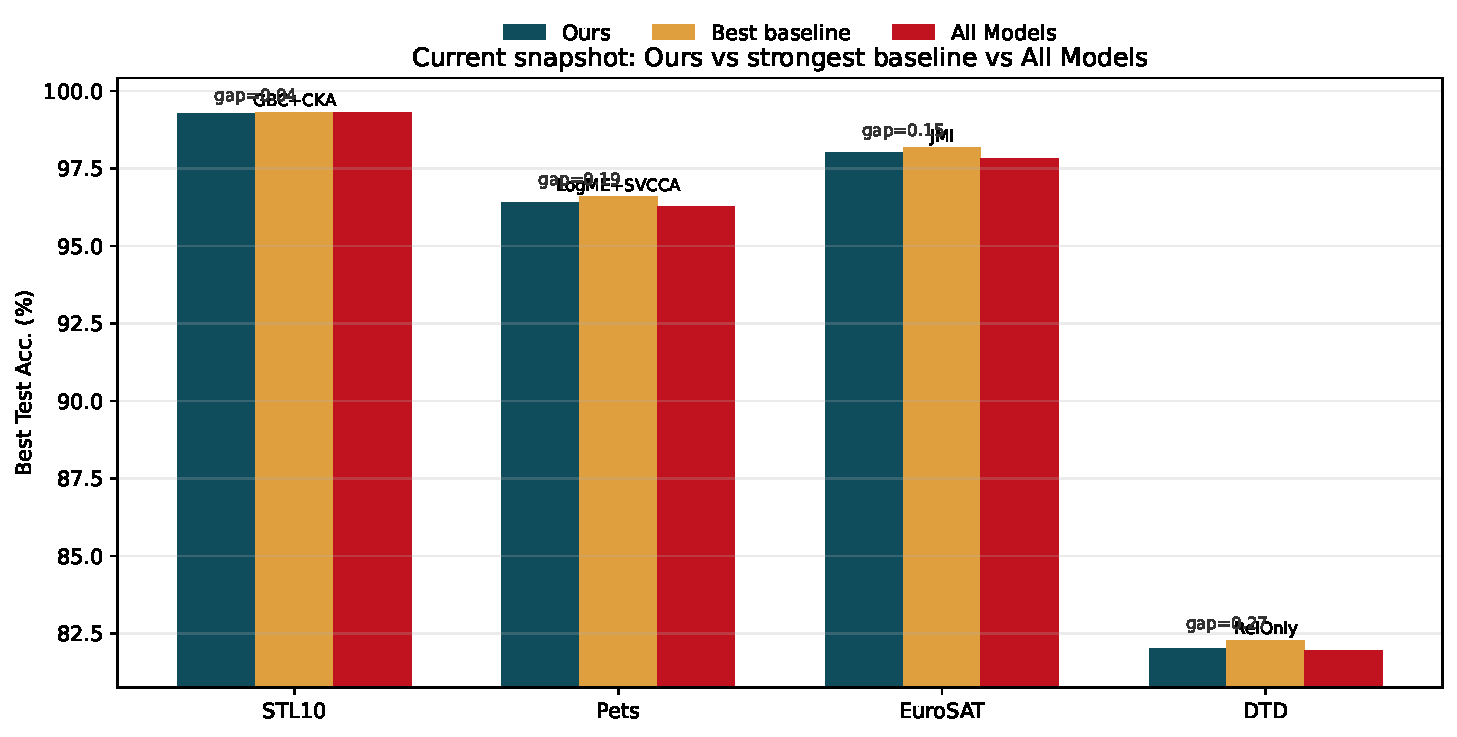
\includegraphics[width=\textwidth]{generated/current_selection_bar_chart.pdf}
\caption{Current snapshot on the completed datasets. For each dataset, we compare the current two-term method, the strongest finished baseline, and the no-selection All Models result using their best finished test accuracy.}
\label{fig:current-selection-bar}
\end{figure}

\section{哪些地方是严格证明，哪些地方只是带条件或近似}

\paragraph{严格可证的部分}
\begin{itemize}
    \item Bayes 风险对特征扩充单调不增；
    \item 互信息对特征扩充单调不减；
    \item 测试风险的精确分解；
    \item 单步性能退化的充要条件；
    \item 边际标签信息的三项精确分解。
\end{itemize}

\paragraph{带条件成立的部分}
\begin{itemize}
    \item “准确率先上升后下降”需要附加假设：边际收益递减、边际代价递增并最终跨越；
    \item “存在最优模型数”不是无条件普适定理，而是针对 few-shot 融合的合理结构假设下成立。
\end{itemize}

\paragraph{工程近似与实验协议的部分}
\begin{itemize}
    \item $\widehat R$ 不是互信息本身，只是相关性的代理；
    \item CKA 不是 $I(F_m; F_S)$ 的无偏估计，只是冗余代理；
    \item 第三项采用 pairwise low-order approximation，而不是 set-level 条件互信息的直接估计；
    \item PCA + 类条件高斯估计器是可计算近似，不是严格一致估计；
    \item class-conditional CKA 只是探索性诊断，不能替代第三项。
    \item 经验评估采用 train/val/test 协议，其中 test 只用于最终一次报告。
\end{itemize}

\begin{thebibliography}{20}

\bibitem{bartlett2002rademacher}
P.~L. Bartlett and S.~Mendelson.
\newblock Rademacher and Gaussian complexities: Risk bounds and structural results.
\newblock {\em Journal of Machine Learning Research}, 3:463--482, 2002.

\bibitem{kawaguchi2023does}
K.~Kawaguchi, Z.~Deng, X.~Ji, and J.~Huang.
\newblock How does information transfer in deep neural networks?
\newblock In {\em Proceedings of the 40th International Conference on Machine Learning (ICML)}, 2023.

\bibitem{krause2008near}
A.~Krause, A.~Singh, and C.~Guestrin.
\newblock Near-optimal sensor placements in {G}aussian processes: Theory, efficient algorithms and empirical studies.
\newblock {\em Journal of Machine Learning Research}, 9:235--284, 2008.

\bibitem{nemhauser1978analysis}
G.~L. Nemhauser, L.~A. Wolsey, and M.~L. Fisher.
\newblock An analysis of approximations for maximizing submodular set functions---{I}.
\newblock {\em Mathematical Programming}, 14(1):265--294, 1978.

\bibitem{hughes1968mean}
G.~F. Hughes.
\newblock On the mean accuracy of statistical pattern recognizers.
\newblock {\em IEEE Transactions on Information Theory}, 14(1):55--63, 1968.

\bibitem{gretton2005measuring}
A.~Gretton, O.~Bousquet, A.~Smola, and B.~Sch{\"o}lkopf.
\newblock Measuring statistical dependence with {H}ilbert-{S}chmidt norms.
\newblock In {\em Proceedings of the 16th International Conference on Algorithmic Learning Theory (ALT)}, pages 63--77, 2005.

\bibitem{kornblith2019similarity}
S.~Kornblith, M.~Norouzi, H.~Lee, and G.~Hinton.
\newblock Similarity of neural network representations revisited.
\newblock In {\em Proceedings of the 36th International Conference on Machine Learning (ICML)}, pages 3519--3529, 2019.

\bibitem{brown2012conditional}
G.~Brown, A.~Pocock, M.-J. Zhao, and M.~Luj{\'a}n.
\newblock Conditional likelihood maximisation: A unifying framework for information theoretic feature selection.
\newblock {\em Journal of Machine Learning Research}, 13:27--66, 2012.

\bibitem{tishby2000information}
N.~Tishby, F.~C. Pereira, and W.~Bialek.
\newblock The information bottleneck method.
\newblock {\em arXiv preprint physics/0004057}, 2000.

\bibitem{you2021logme}
K.~You, Y.~Liu, J.~Wang, and M.~Long.
\newblock Log{ME}: Practical assessment of pre-trained models for transfer learning.
\newblock In {\em Proceedings of the 38th International Conference on Machine Learning (ICML)}, pages 12133--12143, 2021.

\bibitem{nguyen2020leep}
C.~Nguyen, T.~Hassner, M.~Seez, and C.~Archambeau.
\newblock {LEEP}: A new measure to evaluate transferability of learned representations.
\newblock In {\em Proceedings of the 37th International Conference on Machine Learning (ICML)}, pages 7294--7305, 2020.

\bibitem{pandy2022transferability}
S.~Pandy, A.~Agostinelli, and J.~Uijlings.
\newblock Transferability estimation using {B}hattacharyya class separability.
\newblock In {\em Proceedings of the IEEE/CVF Conference on Computer Vision and Pattern Recognition (CVPR)}, pages 9172--9182, 2022.

\bibitem{bao2019information}
Y.~Bao, Y.~Li, S.-L. Huang, L.~Zhang, L.~Zheng, A.~Zamir, and L.~Guibas.
\newblock An information-theoretic approach to transferability in task transfer learning.
\newblock In {\em Proceedings of the 26th International Conference on Machine Learning (ICML)}, pages 2309--2318, 2019.

\bibitem{raghu2017svcca}
M.~Raghu, J.~Gilmer, J.~Yosinski, and J.~Sohl-Dickstein.
\newblock {SVCCA}: Singular vector canonical correlation analysis for deep learning dynamics and interpretability.
\newblock In {\em Advances in Neural Information Processing Systems (NeurIPS)}, pages 6076--6085, 2017.

\end{thebibliography}

\end{document}
